La representación gráfica de la posición y la velocidad revela un ciclo límite con un mínimo de error, un comportamiento típico documentado en la referencia [Diana]. A continuación, se presentan las gráficas correspondientes de posición y velocidad.
Con el diseño del controlador [tal] se muestran.\\

Se observa como la acción de control hace que el sistema entre en un ciclo límite, lo que significa que el levitador oscila alrededor de la posición de referencia.
% \begin{figure}[htbp]
%     \centering
%     \caption{Velocidad y posición}
%     \label{friccionlineal}
% \end{figure}
\begin{figure}[h]
    \centering
       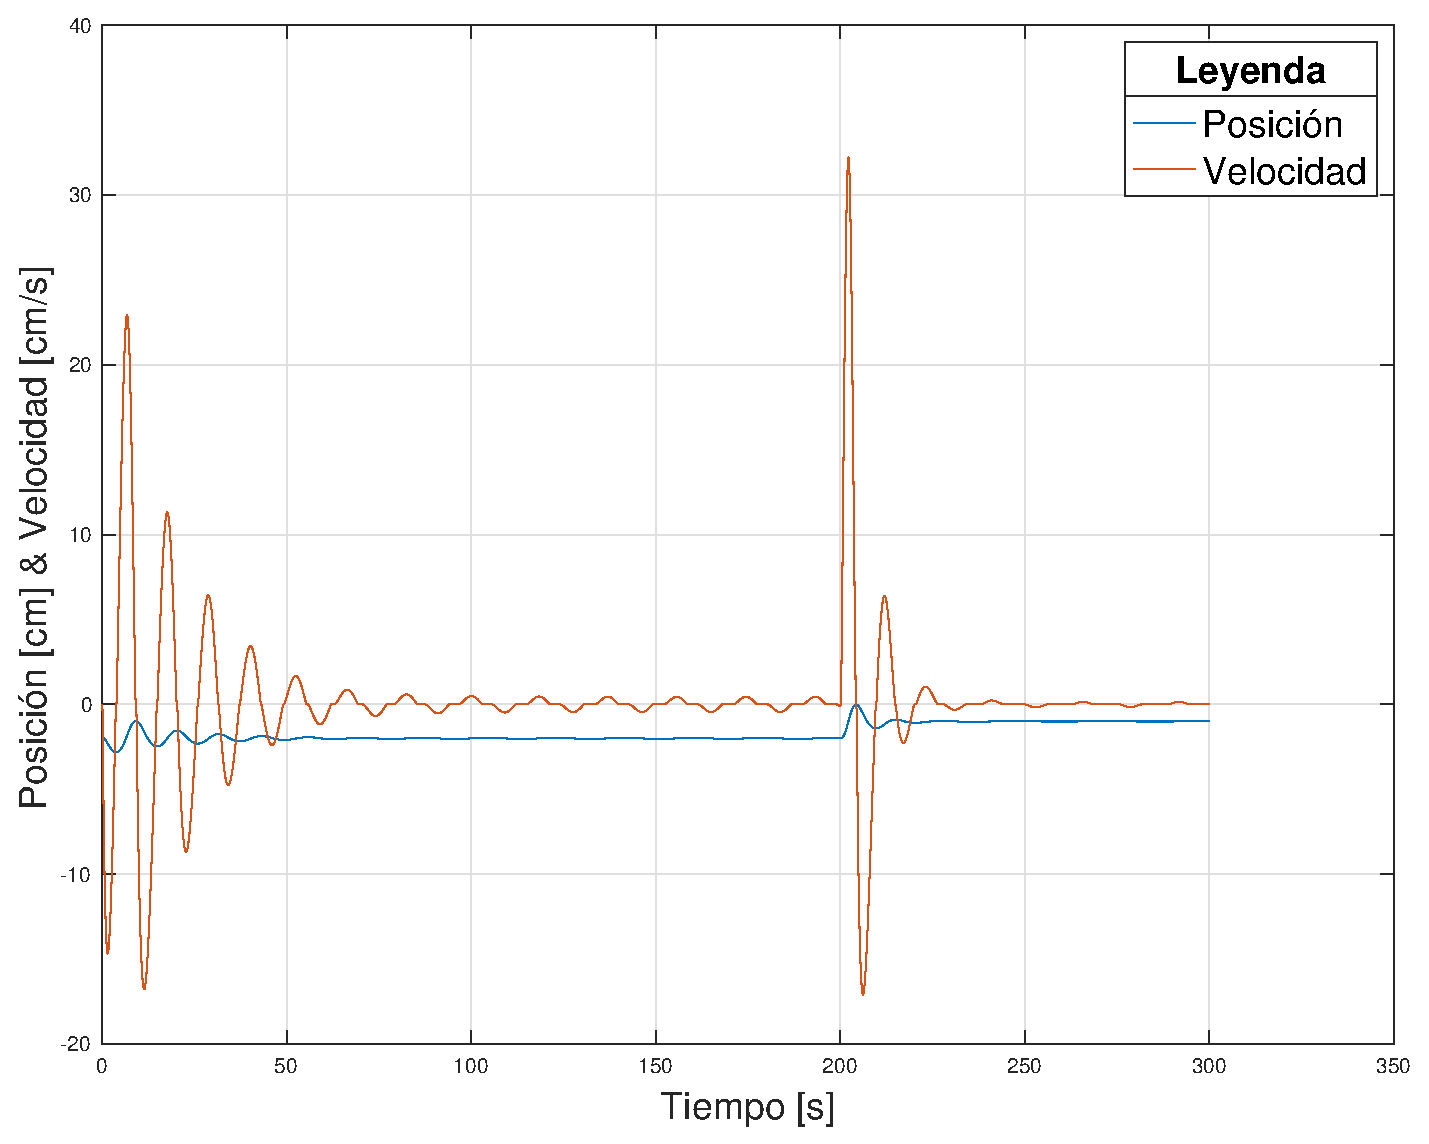
\includegraphics[width=0.6\textwidth]{images/posicionyvelocidad.eps}
    \caption{Posición y velocidad}
    \label{posicionyvelocidad}
\end{figure}
\newpage

Se observa que el error no es necesariamente cero. A pesar de ello se observan excelentes resultados.
\begin{figure}[hb]
    \centering
       \includegraphics[width=0.6\textwidth]{figura2.eps}
    \caption{error}
    \label{error}
\end{figure}

\newpage

Los resultados en las gráficas de voltaje de control antes y después del efecto stick-slip  muestran en primera instancia que el controlador cumple con los requisitos técnicos de la fuente de voltaje para mantener el disco levitando.
\begin{figure}[hb]
    \centering
       \includegraphics[width=0.6\textwidth]{figura3.eps}
    \caption{error}
    \label{error}
\end{figure}

\newpage
\begin{center}
  \tikzstyle{startstop} = [rectangle, rounded corners, minimum width=3cm, minimum height=1cm, text centered, draw=black, fill=red!30]
  \tikzstyle{io} = [trapezium, trapezium left angle=70, trapezium right angle=110, minimum width=3cm, minimum height=1cm, text centered, draw=black, fill=blue!30]
  \tikzstyle{process} = [rectangle, minimum width=3cm, minimum height=1cm, text centered, draw=black, fill=orange!30]
  \tikzstyle{decision} = [diamond, minimum width=3cm, minimum height=1cm, text centered, draw=black, fill=green!30]
  \tikzstyle{arrow} = [thick,->,>=stealth]
  
  \begin{tikzpicture}[node distance=2cm]
    \node (b1) [startstop] {Start};
    \node(b2)[io, below of=b1, yshift=-0.1cm, align=center]{Condiciones \\ iniciales};
    \node (b3) [decision, below of=b2, yshift=-0.5cm, align=center] {Referencia};
    \node (b4) [process, below of=b3, yshift=-0.5cm] {Controlador};
    \node (b5) [decision, below of=b4, yshift=-0.5cm, align=center] {Zona\\ muerta};
    \node (b6) [process, below of=b5, yshift=-0.5cm] {Planta};
    \node (b7) [startstop, below of=b6, xshift=-4cm, yshift=-0.1cm] {Stop};
    \node (b8) [io,below of=b6, yshift=-0.1cm] {Salida};

    \draw[arrow](b1) -- (b2);
    \draw[arrow](b2) -- (b3);
    \draw[arrow](b3) -| node[anchor=south, xshift=1cm] {sí} (b7);
    \draw[arrow](b3) -- node[anchor=west] {no}  (b4);
    \draw[arrow](b4) -- (b5);
    \draw[arrow](b5) -- node[anchor=west] {no, $u_c$} (b6);
    \draw[arrow](b5) -- node[anchor=south, xshift=0.6cm] {sí, $u_{zm}$} (b5 -| b6.east) -- ++(1,0) |- (b6.east);
    \draw[arrow](b6) -- (b8);
    \draw[arrow](b8) -- (b8 -| b3.east) -- ++(2,0) |- (b3.east);
  \end{tikzpicture}
\end{center}



% \begin{figure}[htbp]
%     \centering
%     \includegraphics[width=0.6\textwidth]{images/chapter_6/figura2.eps}
%     \caption{Voltaje de control antes y después de la zona muerta}
%     \label{Votaje antes y después de Zona Muerta}
% \end{figure}

% \begin{figure}[htbp]
%     \centering
%     \includegraphics[width=0.6\textwidth]{images/chapter_6/figura3.eps}
%     \caption{Fricción lineal}
%     \label{errorDeadZonaNoLinealFriction}
% \end{figure}

% \newpage

% \begin{figure}[ht]
%     \centering
%     \includegraphics[width=0.6\textwidth]{images/chapter_6/position.eps}
%     \caption{Fricción lineal}
%     \label{position}
% \end{figure}